\documentclass[11pt, a4paper, reqno]{scrartcl}

\usepackage[utf8]{inputenc}
\usepackage[T1]{fontenc}
\usepackage{a4wide}
\usepackage{dejavu}
\usepackage{graphicx}
\usepackage{listings}
\usepackage{xcolor}
\usepackage{float}
\usepackage{amsmath}
\usepackage{microtype}

% for latex output of pandas
\usepackage{booktabs}

\lstset{
	language=R,
	backgroundcolor=\color{gray!5},
	numbers=left,
	captionpos=t,
	breaklines=true,
	frame=l,
	xleftmargin=\parindent,
	basicstyle=\linespread{1.2}\footnotesize\ttfamily,
	keywordstyle=\bfseries\color{blue!50!black},
	commentstyle=\itshape\color{purple!40!black},
	identifierstyle=\color{teal!50!black},
	stringstyle=\color{red},
	alsoletter={_},
	otherkeywords={!,!=,~,*,\&,\%/\%,\%*\%,\%\%,<-,<<- }
}

\begin{document}
    \title{Computational Statistics and Data Analysis\\Sheet No. 6}
    \author{David Bubeck, Patrick Nisbl\`e}
    \maketitle
    \section{Correlated Variables}
    \begin{align}
        \bar V_1 = 6.991867\\
        \bar V_2 = 9.009960
    \end{align}
    We calculated the following two matrices:
    \begin{align}
        \text{covariance matrix }C_{ij} = \begin{pmatrix}
            5.045109 & 1.508497\\
            1.508497 & 1.492933
        \end{pmatrix}\\
        \text{correlation matrix }C_{ij} = \begin{pmatrix}
            1.0000000 & 0.5496535\\
            0.5496535 & 1.0000000
        \end{pmatrix}
    \end{align}
    
    using following code:
    \begin{figure}[H]
        \lstinputlisting[lastline=46]{Exercise06_1.r}
    \end{figure}
    \begin{figure}
        \lstinputlisting[firstline=48]{Exercise06_1.r}
    \end{figure}

    resulting in:
    \begin{figure}[H]
        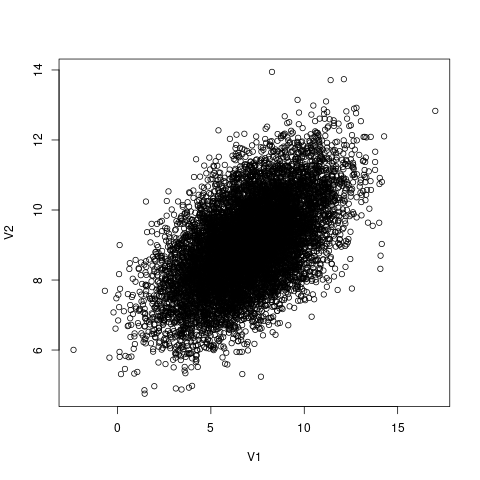
\includegraphics[height=0.4\paperheight]{dataPlot.png}
        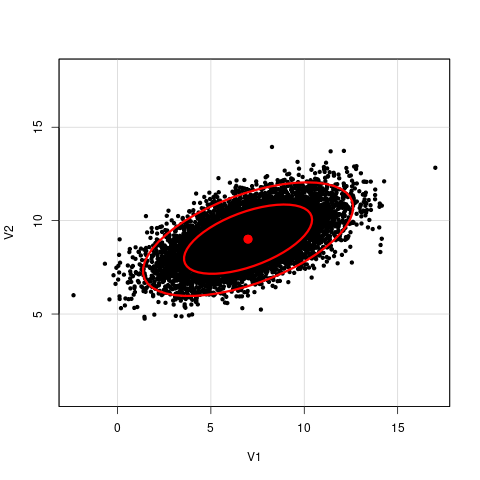
\includegraphics[height=0.4\paperheight]{ellipsesPlot.png}
    \end{figure}
	% !TeX root = sheet6_solution.tex
\section{Non-uniform distributions}
using the following code we plotted $p(\theta,g)$ und $p(\eta,g)$, as well as performed sampling with g=0.5

\begin{figure}[H]
	\lstinputlisting{p2.r}
\end{figure}
\begin{figure}[H]
    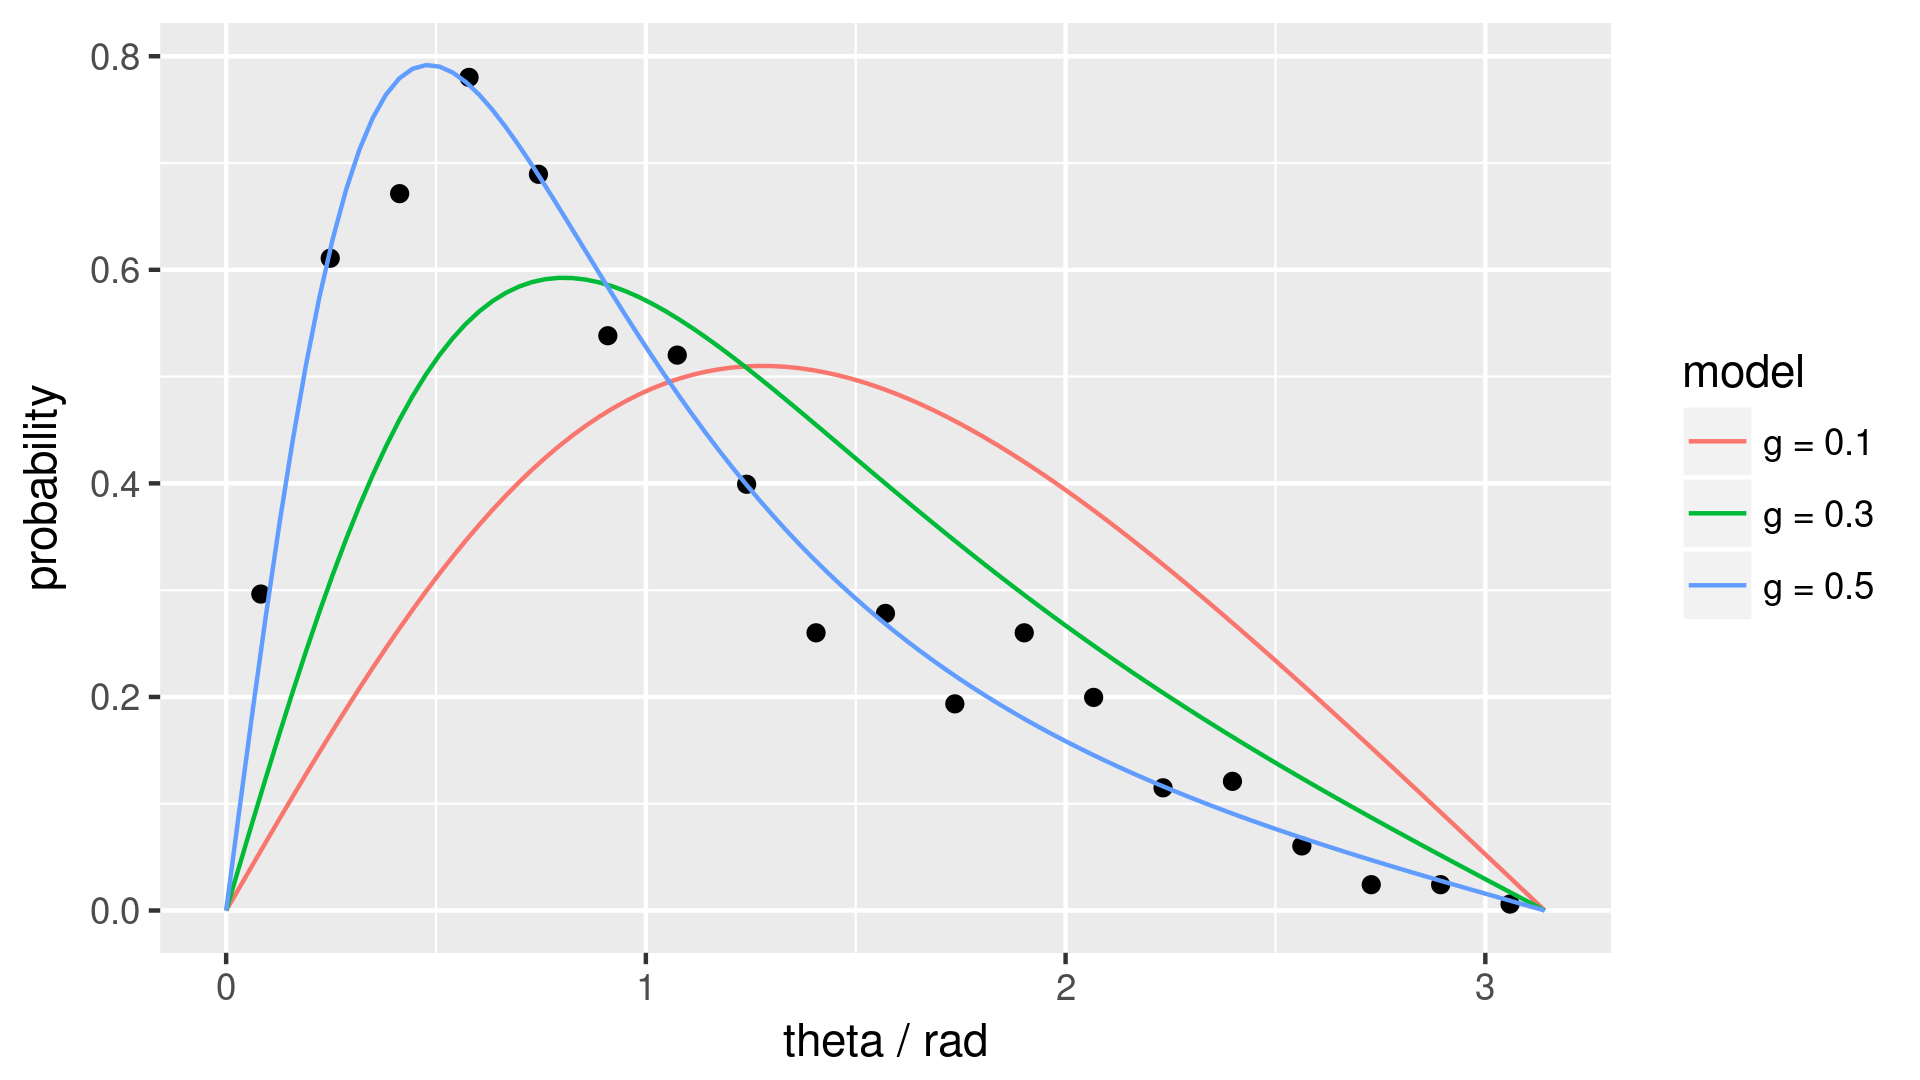
\includegraphics[]{6-2_scatter_prob_b}
\end{figure}
\begin{figure}[H]
    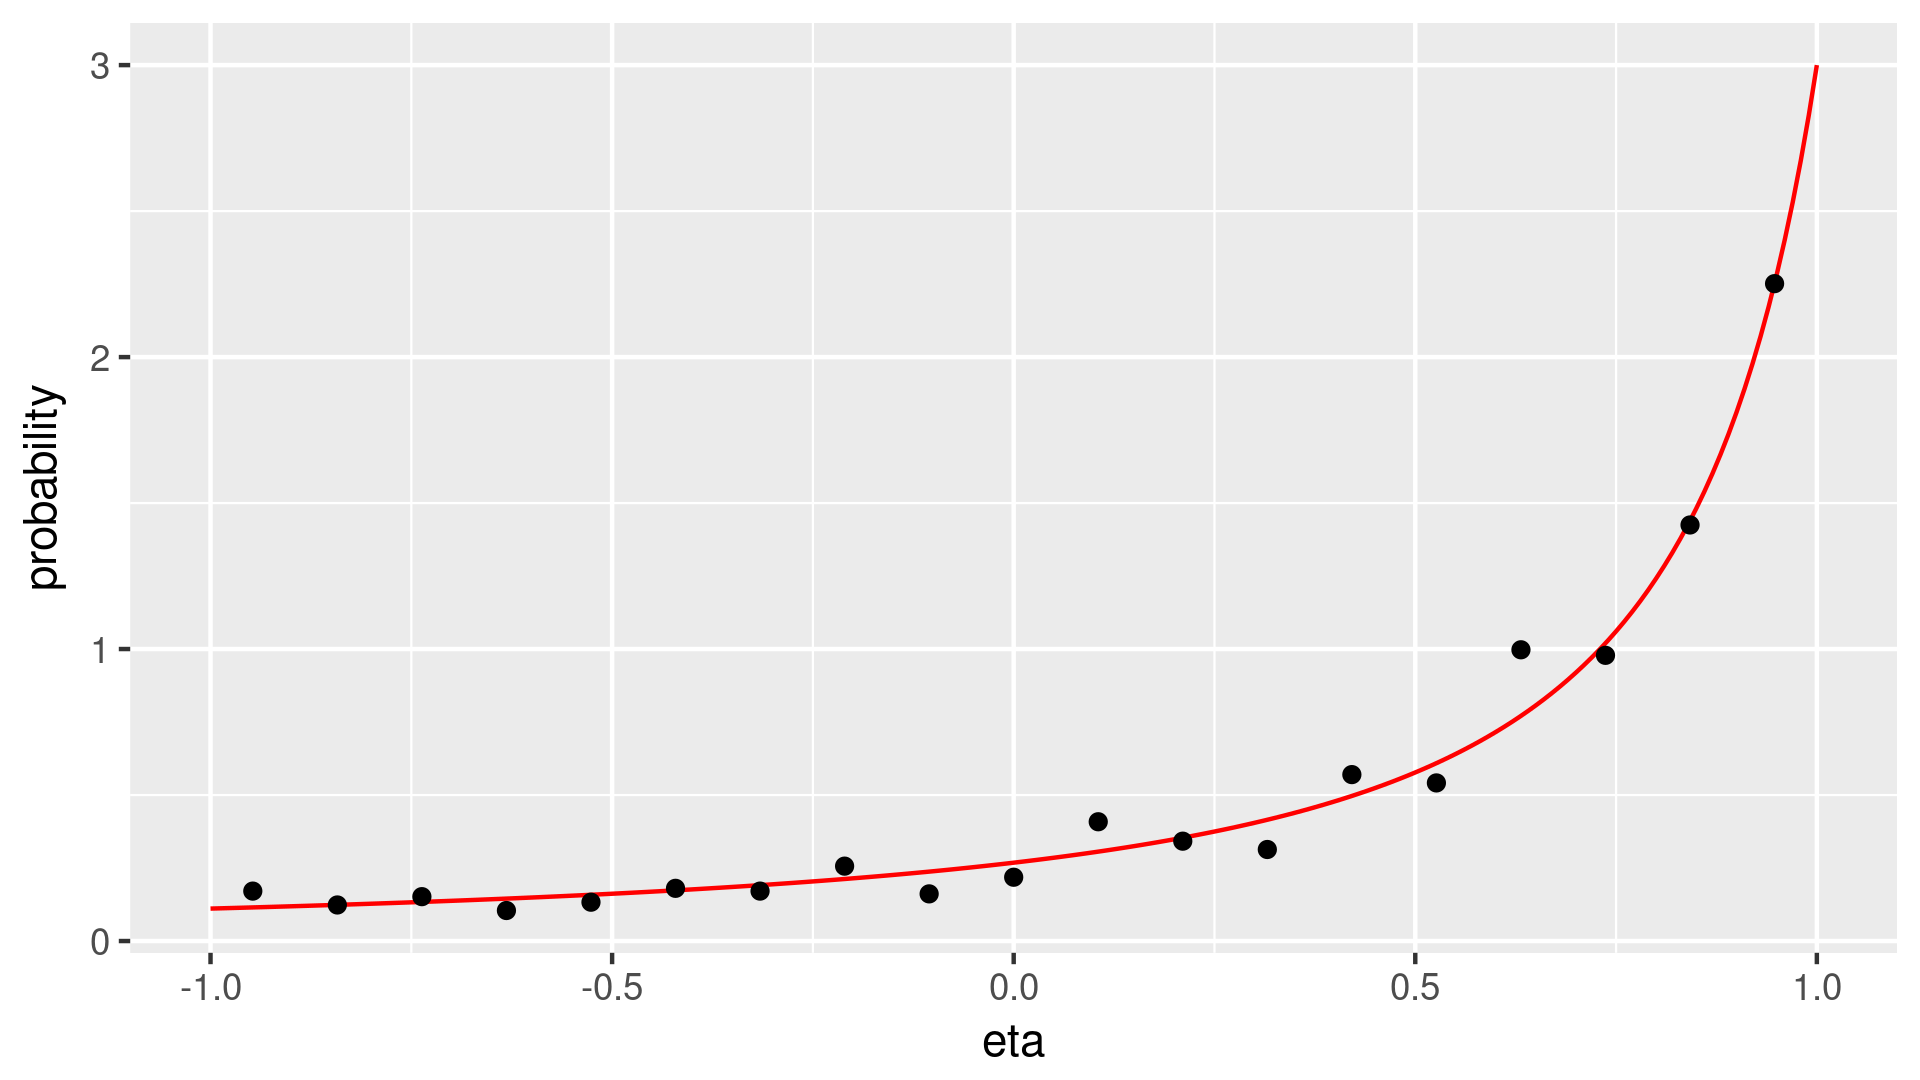
\includegraphics[]{6-2_scatter_eta_b}
\end{figure}
	% !TeX root = sheet6_solution.tex
\section{Higher order moments of multivariate Gaussian}
\begin{align}
	E[x_1\cdot x_2\cdot\dots x_{2n}] = \sum_1^{\binom{2n}{2}}\left( \prod_{1}^{n} E[x_ix_j] \right)
\end{align}

\subsection{a)}
\begin{align}
	E[x_1^4x_2^2]=&\binom{3}{1}_{perm} 2^0_{rot} E[x_1^2]^2 E[x_2^2]\\
	+&\binom{3}{1}_{perm} 2^2_{rot} E[x_1^2] E[x_1x_2]^2\\
	=&3\sigma_1^4\sigma_2^2 + 12(\varrho_{12}\sigma_1\sigma_2)^2\sigma_1^2\\
\end{align}
\subsection{b)}
\begin{align}
	E[x_1^3x_2]=&\binom{4}{2}E[x_1^2]E[x_1x_2]\\
	=&6\sigma_1^2(\varrho_{12}\sigma_1\sigma_2)
\end{align}

\end{document}